\documentclass[a4paper,UTF8]{article}
\usepackage{ctex}
\usepackage[margin=1.25in]{geometry}
\usepackage{color}
\usepackage{graphicx}
\usepackage{amssymb}
\usepackage{amsmath}
\usepackage{amsthm}
\usepackage{enumerate}
\usepackage{bm}
\usepackage{hyperref}
\usepackage{pgfplots}
\usepackage{epsfig}
\usepackage{color}
\usepackage{tcolorbox}
\usepackage{mdframed}
\usepackage{lipsum}
\newmdtheoremenv{thm-box}{myThm}
\newmdtheoremenv{prop-box}{Proposition}
\newmdtheoremenv{def-box}{定义}

\setlength{\evensidemargin}{.25in}
\setlength{\textwidth}{6in}
\setlength{\topmargin}{-0.5in}
\setlength{\topmargin}{-0.5in}
% \setlength{\textheight}{9.5in}
%%%%%%%%%%%%%%%%%%此处用于设置页眉页脚%%%%%%%%%%%%%%%%%%
\usepackage{fancyhdr}                                
\usepackage{lastpage}                                   
\usepackage{layout}                                     
\newtheorem*{solution}{Solution}

\footskip = 10pt 
\pagestyle{fancy}                    % 设置页眉                 
\lhead{2020年秋季}                    
\chead{高级机器学习}                                                
% \rhead{第\thepage/\pageref{LastPage}页} 
\rhead{作业一}                                                                                               
\cfoot{\thepage}                                                
\renewcommand{\headrulewidth}{1pt}  			%页眉线宽,设为0可以去页眉线
\setlength{\skip\footins}{0.5cm}    			%脚注与正文的距离           
\renewcommand{\footrulewidth}{0pt}  			%页脚线宽,设为0可以去页脚线

\makeatletter 									%设置双线页眉                                        
\def\headrule{{\if@fancyplain\let\headrulewidth\plainheadrulewidth\fi%
\hrule\@height 1.0pt \@width\headwidth\vskip1pt	%上面线为1pt粗  
\hrule\@height 0.5pt\@width\headwidth  			%下面0.5pt粗            
\vskip-2\headrulewidth\vskip-1pt}      			%两条线的距离1pt        
 \vspace{6mm}}     								%双线与下面正文之间的垂直间距              
\makeatother  

%%%%%%%%%%%%%%%%%%%%%%%%%%%%%%%%%%%%%%%%%%%%%%
\numberwithin{equation}{section}
%\usepackage[thmmarks, amsmath, thref]{ntheorem}
\newtheorem{myThm}{myThm}
\newtheorem*{myDef}{Definition}
\newtheorem*{mySol}{Solution}
\newtheorem*{myProof}{Proof}
\newtheorem*{myRemark}{备注}
\renewcommand{\tilde}{\widetilde}
\renewcommand{\hat}{\widehat}
\newcommand{\indep}{\rotatebox[origin=c]{90}{$\models$}}
\newcommand*\diff{\mathop{}\!\mathrm{d}}

\usepackage{multirow}

%--

%--
\begin{document}
\title{高级机器学习\\
作业一}
\author{周韧哲\, 181220076\, zhourz@smail.nju.edu.cn} 
\maketitle
%%%%%%%% 注意: 使用XeLatex 编译可能会报错,请使用 pdfLaTex 编译 %%%%%%%

\section*{学术诚信}

本课程非常重视学术诚信规范,助教老师和助教同学将不遗余力地维护作业中的学术诚信规范的建立。希望所有选课学生能够对此予以重视。\footnote{参考尹一通老师\href{http://tcs.nju.edu.cn/wiki/}{高级算法课程}中对学术诚信的说明。}

\begin{tcolorbox}
	\begin{enumerate}
		\item[(1)] 允许同学之间的相互讨论,但是{\color{red}\textbf{署你名字的工作必须由你完成}},不允许直接照搬任何已有的材料,必须独立完成作业的书写过程;
		\item[(2)] 在完成作业过程中,对他人工作(出版物、互联网资料)中文本的直接照搬(包括原文的直接复制粘贴及语句的简单修改等)都将视为剽窃,剽窃者成绩将被取消。{\color{red}\textbf{对于完成作业中有关键作用的公开资料,应予以明显引用}};
		\item[(3)] 如果发现作业之间高度相似将被判定为互相抄袭行为,{\color{red}\textbf{抄袭和被抄袭双方的成绩都将被取消}}。因此请主动防止自己的作业被他人抄袭。
	\end{enumerate}
\end{tcolorbox}

\section*{作业提交注意事项}
\begin{tcolorbox}
	\begin{enumerate}
		\item[(1)] 请在LaTeX模板中{\color{red}\textbf{第一页填写个人的姓名、学号、邮箱信息}};
		\item[(2)] 本次作业需提交该pdf文件、问题3可直接运行的源码(学号\_.py),将以上两个文件压缩成zip文件后上传。zip文件格式为{\color{red}\textbf{学号.zip}},例如170000001.zip;pdf文件格式为{\color{red}\textbf{学号\_姓名.pdf}},例如170000001\_张三.pdf。
		\item[(3)] 未按照要求提交作业,或提交作业格式不正确,将会{\color{red}\textbf{被扣除部分作业分数}};
		\item[(4)] 本次作业提交截止时间为{\color{red}\textbf{11月8日23:59:59}}。除非有特殊情况(如因病缓交),否则截止时间后不接收作业,本次作业记零分。
	\end{enumerate}
\end{tcolorbox}

\newpage
\section{[30pts] VC Dimensions}
本题探讨~VC~维的性质。

\begin{enumerate}[(1)]
	\item \textbf{[10pts]} 请在样本空间~$\mathcal{X} = [0,1]$~上构造一个有限假设空间~$\mathcal{H}$~使得~$\mbox{VC}(\mathcal{H}) = \left \lfloor \log_2(\left| \mathcal{H} \right| ) \right \rfloor $.
	\item \textbf{[10pts]} 定义轴平行四边形概念类~$\mathcal H = \{h_{(a_1, a_2, b_1, b_2)}(x, y): a_1\le a_2 \land b_1\le b_2\}$, 其中
	\[ h_{(a_1, a_2, b_1, b_2)}(x, y) = \begin{cases}
	1&\quad \text{ if } a_1\le x\le a_2 \land b_1\le y \le b_2 \\
	0 & \quad \text{otherwise}
	\end{cases}
	\]
	请证明~$\mathcal H$~的~VC~维为~4.
	\item \textbf{[10 pts]} 请证明最近邻分类器的假设空间的~VC~维可以为无穷大.
\end{enumerate}

\begin{solution}.
\begin{enumerate}[$(1)$]
	\item 令$$\mathcal{H}=\{h_{[0,\frac{1}{4}]},h_{[0,\frac{1}{2}]},h_{[\frac{1}{3},\frac{2}{3}]},h_{[\frac{1}{2},1]}\}$$
	则$|\mathcal{H}|=4$。对于$x\in\mathcal{X},h_{[a,b]}\in\mathcal{H}$,若$x\in [a,b]$,则$h_{[a,b]}(x)=1$,否则$h_{[a,b]}(x)=-1$。则存在$x_1=0.2,x_2=0.35$,该假设空间$\mathcal{H}$可以将其打散。但是对任意大小为$3$的示例集$\{x_3,x_4,x_5\}$,不妨设$x_3<x_4<x_5$,则不存在假设能对分结果
	$\{(x_3,1),(x_4,-1),(x_5,1)\}$。所以$VC(\mathcal{H})=2=\left \lfloor \log_2(\left| \mathcal{H} \right| ) \right \rfloor$。
	\item 取$\mathbb{R}^2$中四个点$\{(-1,0),(0,1),(1,0),(0,-1)\}$,容易看出$\mathcal{H}$能打散该集合(五大类情况):标签为一个$1$三个$0$的$h_{(-0.5,0.5,0.5,1.5)}$,标签为两个$1$两个$0$的:$h_{(-1,0,0,1)},h_{(-1,1,-0.5,0.5)}$,标签为三个$1$一个$0$的$h_{(-1,1,0,1)}$,标签全为$1$的$h_{(-1,1,-1,1)}$,标签全为$0$的$h_{100,120,100,120}$。由几何关系容易知道$\mathcal{H}$中存在假设能使得该示例集取遍所有标签。
	      \\取示例集$\{(x_i,y_i)|i=1,2,3,4,5\}$,令
	      \begin{align*}
	      	x^*&=\max\{x_i|i=1,2,3,4,5\},\quad
	      	x_*=\min\{x_i|i=1,2,3,4,5\}\\
	      	y^*&=\max\{y_i|i=1,2,3,4,5\},\quad
	      	y_*=\min\{y_i|i=1,2,3,4,5\}
	      \end{align*}
          得到四个点构成的集合$\mathcal{M}=\{(x_*,y_*),(x_*,y^*),(x^*,y_*),(x^*,y^*)\}$构成了包围该示例集的矩形。我们在该矩形的四条边中各取一个点:如果示例集中有多个点在一条边上,则任取一个;若没有点,则不取。这样的点集$\mathcal{A}$必然非空,否则该矩形就可以“压缩”直到有点出现在边上。
	      令取出来的点标记为$1$,其他点标记为$0$,则没有任何假设能够实现这种对分结果,因为当某个假设h使得在$\mathcal{A}$中的点划分为$1$时,其构成的矩形必然也包括了示例集中不在$\mathcal{A}$中的点,从而被划分为$1$,无法被h划分为$0$。
	 \item 取大小为n的示例集$\{x_i|i=1\cdots,n)\}$,最近邻分类器会将训练集的每个样本标记为其类别,(与x距离最近的点就是x本身),x的类别可以是任意的,所以最近邻分类器的假设空间可以打散任意大小的示例集,因此VC维为无穷大。
\end{enumerate}
\end{solution}

\section{\textbf{[40pts]} Understanding the Parameters in LVW from A Probabilistic Perspective}
课程中,我们介绍了一种包裹式特征选择算法Las Vegas Wrapper(简称LVW),该算法的流程如教材中图11.1所示。首先请各位回顾一下LVW算法,接下来我们将对一种特殊情况下的LVW做一些分析,过程中复习一些简单的概率知识,并从更理性的角度理解LVW中的参数。

现在,我们获得了一个数据集$D$,该数据集中一共包含$N$个特征,设特征集合为$A=\{f_1,f_2,\cdots,f_N\}$。我们知道,对于某个具体任务,特征的质量参差不齐,高质量的特征会带来高质量的性能,低质量的特征会带来低质量的性能。我们设第$i$个特征的质量为$2^{i-1}$,即$N$个特征的质量分别为$1,2,4,\cdots,2^{N-1}$。我们规定:给定一个特征子集$A^\prime$,学习器在$A^\prime$上的性能恰好等于$A^\prime$中包含的所有特征的质量之和。设特征子集$A^\prime$中特征的质量之和记作$Q(A^\prime)$。

\begin{enumerate}[(1)]
\item \textbf{[5pts]} 现执行一次图11.1中第$6$行的语句,产生一个特征子集$A^\prime$,试求数学期望$\mathbb{E}[Q(A^\prime)]$。

\item \textbf{[10pts]} 现在,LVW算法已经执行了一段时间了,当前得到的最优特征子集为$B$,我们记$R=Q(B)$。设函数$better(n,r)$表示从前$n$个特征中随机产生一个特征子集且该特征子集的质量大于$r$的概率。试求$better(N,R)$。这里我们允许以递归式和递归边界来表达$better(N,R)$。
    
\item \textbf{[10pts]} 从现在开始,我们设$better(n,r)$是一个已知函数。在LVW算法中,当连续$T$个随机生成的子集不比当前的最优子集更好时,算法结束。我们仍然设当前得到的最优特征子集为$B$,$B$的质量为$R=Q(B)$。在本小问中,我们还设$T$是一个已知参数。设布尔型随机变量$e$,$p(e=1|T)$表示经过恰好$T$次循环后LVW算法结束的概率,$p(e=0|T)$表示经过恰好$T$次循环后LVW算法没有结束的概率。试求分布$p(e|T)$。

\item \textbf{[5pts]} 由第(3)小问可见,参数$T$越大,LVW算法结束就越([回答“容易”或“困难”]);当前最优子集质量越高,LVW算法结束就越([回答“容易”或“困难”])。

\item \textbf{[10pts]} 现在,我们引入Bayes观点,认为参数$T$是服从某个先验分布$p(T)$的随机变量,且是未知的。我们仍然设当前得到的最优子集为$B$,$B$的质量为$R=Q(B)$。现在,LVW算法继续执行,在恰好执行了$T$个循环后成功退出了。如果我们设$T$的先验分布为整数区间$[1, 10]$上的均匀分布,请对$T$做最大后验估计。这与最大似然估计的结果相同吗?为什么?

\item \textbf{[Bonus 5pts]} 现在,设随机变量$T$只能在$\{1,2,3\}$中取值,且小明设置了一个先验$p(T)$。小红观察到,当前得到的最优子集为$B$,$B$的质量为$R=Q(B)$,且LVW在执行恰好$T$个循环后成功退出了,于是小红试图对$T$做最大后验估计。小红发现,$T$的后验概率在$\{1,2,3\}$上是均匀的,那么小明设置的先验$p(T)$有可能为:(填写一种可能的答案即可)

\end{enumerate}

\begin{solution}.
\begin{enumerate}[$(1)$]
	\item 从伪代码可以看出特征子集必然非空,令其非空子集集合为$\mathcal{A}$,则$|\mathcal{A}|=\sum_{i=1}^{N}\tbinom{N}{i}=2^N-\tbinom{N}{0}=2^N-1$。用向量如$(1,0,1,\cdots,0)$来表示特征的选择情况,第$i$位的$1$表示被选择,$0$表示未被选择,每个特征被选择的概率独立且为$\frac{1}{2}$,则
	\begin{align*}
	 \mathbb{E}[Q(A')]=\sum_{A'\in\mathcal{A}}P(A')Q(A')=\frac{1}{2^N-1}\sum_{A'\in\mathcal{A}}Q(A')
	\end{align*}
    在$\mathcal{A}$中每个特征出现次数为$2^{N-1}$( 固定第$i$个特征被选择,第$i$个特征将会出现$2^{N-1}$次)。所以$\sum_{A'\in\mathcal{A}}Q(A')=2^{N-1}\times(\sum_{i=0}^{N-1}2^i)=2^{N-1}(2^{N}-1)$。从而$\mathbb{E}[Q(A')]=2^{N-1}$。
    \item 一共有$2^N-1$个特征子集,每个特征子集生成的概率相等。由于数列$(1,2,4,\cdots,2^{N-1})$的特殊性,每个特征子集的质量不同,且刚好在$(1,2,3,4,\cdots,2^N-1)$中,其中比R大的有$2^N-1-R$个,因此
    $$better(N,R)=\frac{2^N-1-R}{2^N-1}$$
    \item 令$a=better(N,R)$,这T次循环结束前最优特征子集不变,所以$a$不变,从而分布为:
           \begin{align*}
           &p(e=1|T)=(1-a)^{T},\\
           &p(e=0|T)=a(1-a)^{T-1}
           \end{align*}
    \item 困难;容易。
    \item 显然$T>0$,因为$a\in[0,1)$,所以最大似然估计为$$\arg\max_T (1-a)^T=1$$
          最大后验估计为
          \begin{align*}
          	\arg\max_T &\quad p(T|e=1)\\
          	           &=p(e=1|T)p(T)\\
          	                   &=(1-a)^T\times\frac{1}{10}\\
          	                   &=1
          \end{align*}
          两者结果相同。因为最大后验估计只是比最大似然估计多考虑了一个参数的先验分布,在这里先验分布为均匀分布,也被称为无信息先验,此时最大后验估计等于最大似然估计。
     \item 
         可知$$(1-a)p(1)=(1-a)^2p(2)=(1-a)^3p(3)$$$$p(1)+p(2)+p(3)=1$$
         从而,
         \begin{align*}
         	p(T=1)&=\frac{(1-a)^2}{a^2-3a+3}\\
         	p(T=2)&=\frac{1-a}{a^2-3a+3}\\
         	p(T=3)&=\frac{1}{a^2-3a+3}
         \end{align*}
         \begin{table}
         	\centering
         	\caption{p(T)}
         	\begin{tabular}{|l|l|l|}
         		\hline
         		$p(T=1)$ & $p(T=2)$ & $p(T=3)$ \\ \hline
         		$\frac{(1-a)^2}{a^2-3a+3}$ & $\frac{1-a}{a^2-3a+3}$ & $\frac{1}{a^2-3a+3}$      \\
         		\hline
         	\end{tabular}
         \end{table}\label{table:pT} 
\end{enumerate}
\end{solution}

\section{\textbf{[30pts]} Semi-supervised SVM in practice}
参照教材中图13.4所示的TSVM算法,在所提供的半监督数据集上进行训练,报告模型在未标记数据集以及测试集上的性能。

本次实验的数据集为一个二分类的数据集,已提前划分为训练数据和测试数据,其中训练数据划分为有标记数据和无标记数据。数据的特征维度为30,每一维均为数值类型。数据文件的具体描述如下:
\begin{itemize}
    \item \texttt{label\_X.csv,label\_y.csv}分别是有标记数据的特征及其标签。
    \item \texttt{unlabel\_X.csv,unlabel\_y.csv}分别是无标记数据的特征及其标签。
    \item \texttt{test\_X.csv,test\_y.csv}分别是测试数据的特征及其标签。
\end{itemize}

注意,训练阶段只可以使用\texttt{label\_X.csv,label\_y.csv,unlabel\_X.csv}中的数据,其他的数据只可以在测试阶段使用。
\begin{enumerate}[(1)]
    \item  本次实验要求使用Python3编写,代码统一集中在\texttt{tsvm\_main.py}中,通过运行该文件就可以完成训练和测试,并输出测试结果。
    \item 本次实验需要完成以下功能:
    \begin{itemize}
        \item \textbf{[10pts]} 参照教材中图13.4,使用代码实现TSVM算法。要求:
        \begin{enumerate}[1.]
            \item 不允许直接调用相关软件包中的半监督学习方法。
            \item 可以直接调用相关软件包的SVM算法。
            \item 可以使用诸如\texttt{cvxpy}等软件包求解QP问题。
        \end{enumerate}
        \item \textbf{[10pts]} 使用训练好的模型在无标记数据和测试数据上进行预测,报告模型在这两批数据上的准确率和ROC曲线以及AUC值。
        \item \textbf{[10pts]} 尝试使用各种方法提升模型在测试集上的性能,例如数据预处理,超参数调节等。报告你所采取的措施,以及其所带来的提升。
    \end{itemize}
\end{enumerate}
\begin{solution}.
	\begin{enumerate}[$\bullet$]
		\item 我使用了sklearn的svm模型来实现TSVM算法,最终超参数调节为$C_l=1,C_u=1e-3$,训练得到模型在无标记数据和测试数据上的准确率为$0.9386,0.9558$。同时,为了提升性能,我实现了特征选择算法LVW,令$T=40$,固定随机种子为$3$,得到模型在无标记数据和测试数据上的准确率为$0.9298,0.9823$,auc值为$0.9776,0.9947$。其roc曲线与auc值如下图\ref{fig:unlabel y},图\ref{fig:test y}。
		\begin{figure}[h]
			\centering
			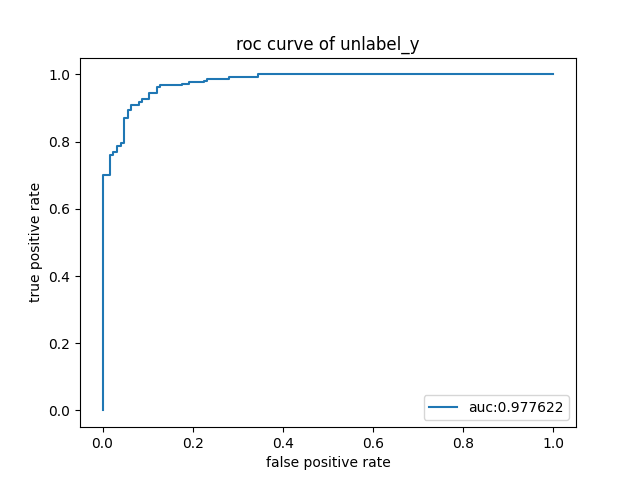
\includegraphics[width=0.8\textwidth]{Figure_1.png}
			\caption{unlabel y}
			\label{fig:unlabel y}
		\end{figure}
	    \begin{figure}[h]
	    	\centering
	    	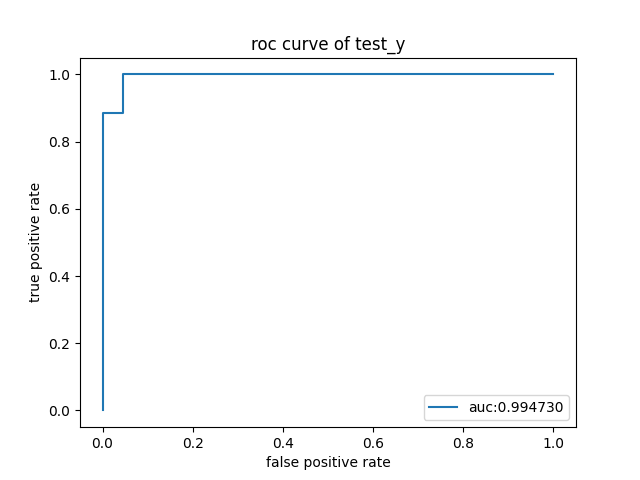
\includegraphics[width=0.8\textwidth]{Figure_2.png}
	    	\caption{test y}
	    	\label{fig:test y}
	    \end{figure}
	\end{enumerate}
\end{solution}
\end{document}